\section{Part C}

The objective of this final part is to simulate the temporal evolution of an incompressible, 2D fluid flow using a projection method. This approach separates the velocity update from pressure correction. The simulation is validated against an analytical solution, allowing for the assessment of accuracy and stability.

\subsection{Algorithm}

The algorithm used follows a projection method, ensuring that the velocity field remains divergence-free at each step. The steps are explained below:

\begin{enumerate}
    \item Initialize physical parameters including the time step and the analytical solution velocity and pressure fields. Calculate initial convective and diffusive terms, time step and R term.
    
    \item Iterate for each timestep until the time limit is reached. For each time iteration:
    \begin{itemize}
        \item Convective and diffusive terms are computed for both velocity components.
        \item Calculate time step for each iteration.
        \item Update R term and use it to find the predictor velocities.
        \item Calculate divergence for predictor velocities.
        \item A Poisson equation for the pseudo P field is solved using the Laplacian matrix.
        \item Calculate pseudo P gradient and substract it from predictor velocities to obtain corrected divergence-free predictor velocities.
        \item Check divergence for predicted and corrected velocity fields. Find maximum values.
        \item Update the iteration velocities with the corrected velocities and and calculate the pressure difference field.
        \item Compute analytical solution.
        \item Store solutions and advance time step.
    \end{itemize}
    \item Calculate errors for each timestep and find maximums.
    \item Visualize results. Plot errors for cell length, compare solutions at a point.
\end{enumerate}

\subsection{Validation Strategy}

At each time iteration, the maximum absolute error between the numerical and analytical solutions is computed over the physical domain for $u$, $v$, and $p$. The evolution of these errors over time shows the accuracy and consistency of the simulation.

The code generates error vs mesh size plots showing that the numerical error decreases with grid refinement. A second-order decay rate in space is expected.

Temporal evolution at a fixed point is compared between analytical and numerical values, confirming that the numerical solution accurately follows the behavior of the analytical one throughout the simulation.

Finally, particle trajectories are simulated through time and displayed in an animation together with velocities. This video is obtained through the code and an image of it is shown in Figure \ref{fig:particlemovement}.

\subsection{Results}

\begin{figure}[H]
    \centering
    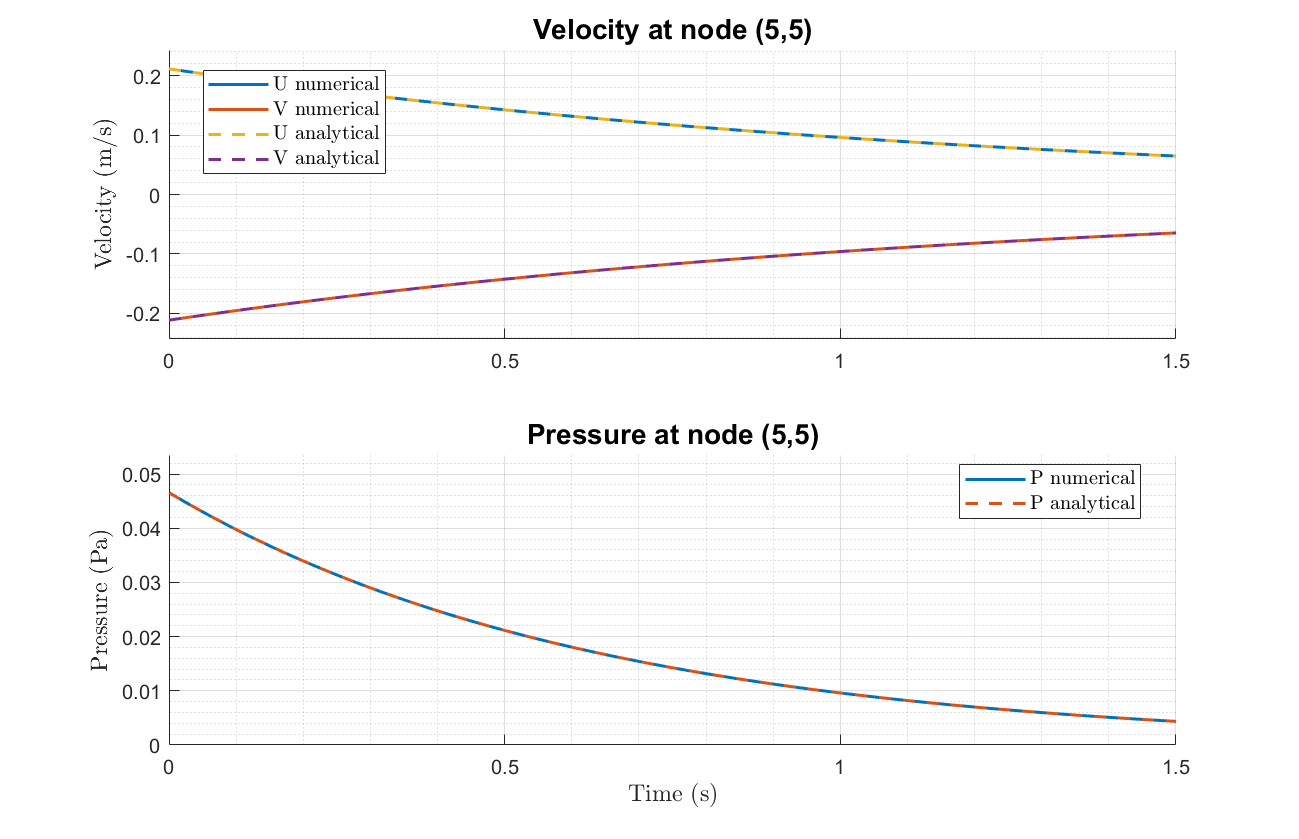
\includegraphics[width=0.6\linewidth]{imatges/comparison.png}
    \caption{Comparison of numerical and analytical calculated values at a point.}
    \label{fig:comparison}
\end{figure}

Figure \ref{fig:comparison} confirmas that the expectation of the numerical solution being a good aproximation of the analytical one is correct.

\begin{figure}[H]
    \centering
    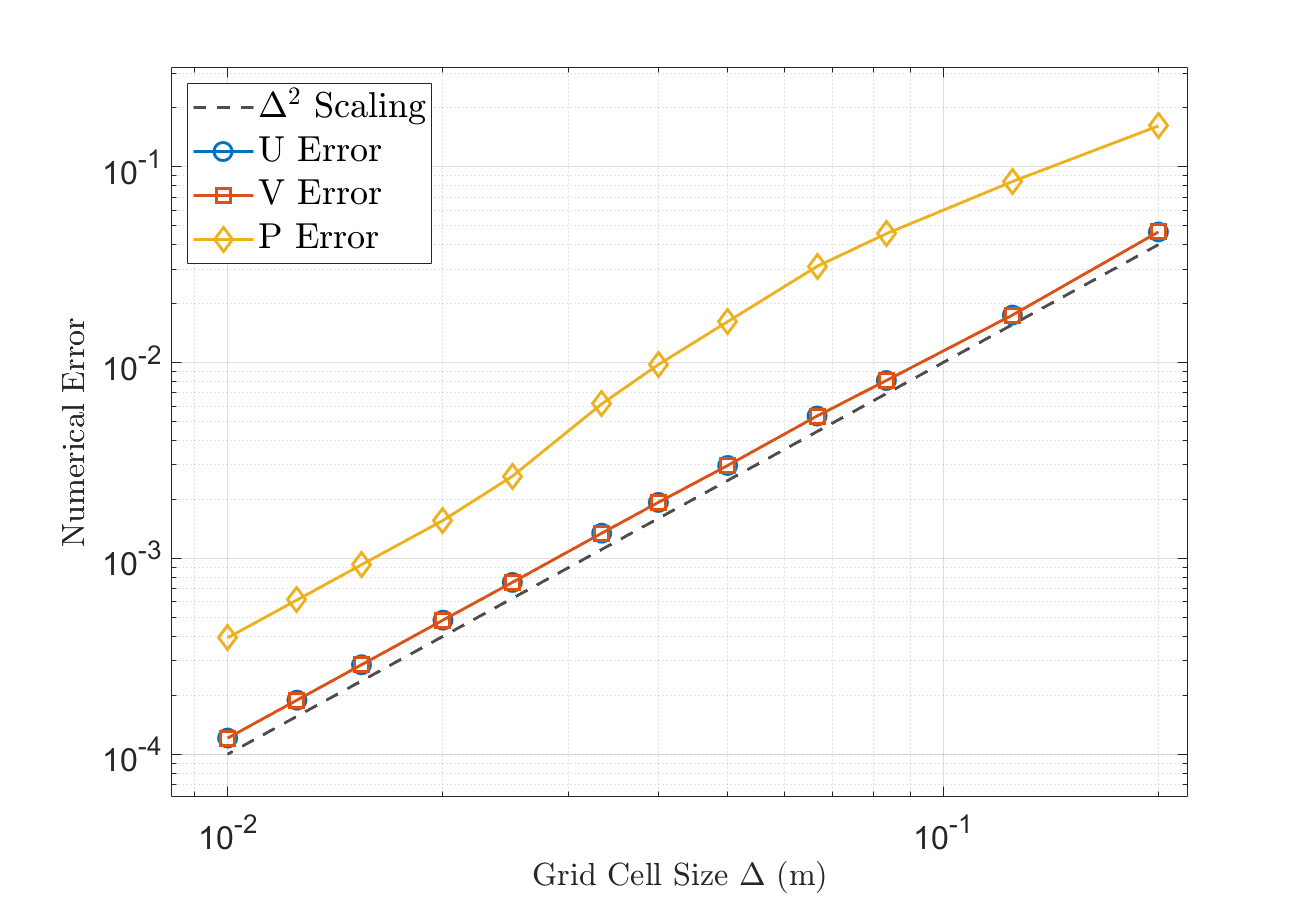
\includegraphics[width=0.6\linewidth]{imatges/partcerror.png}
    \caption{Convergence of error over the mesh.}
    \label{fig:errorC}
\end{figure}

Similarly to the previous parts of the code, the error for the numerical solution for decreasing grid cell size decreases quadratically, confirming second-order accuracy.

\begin{figure}[H]
    \centering
    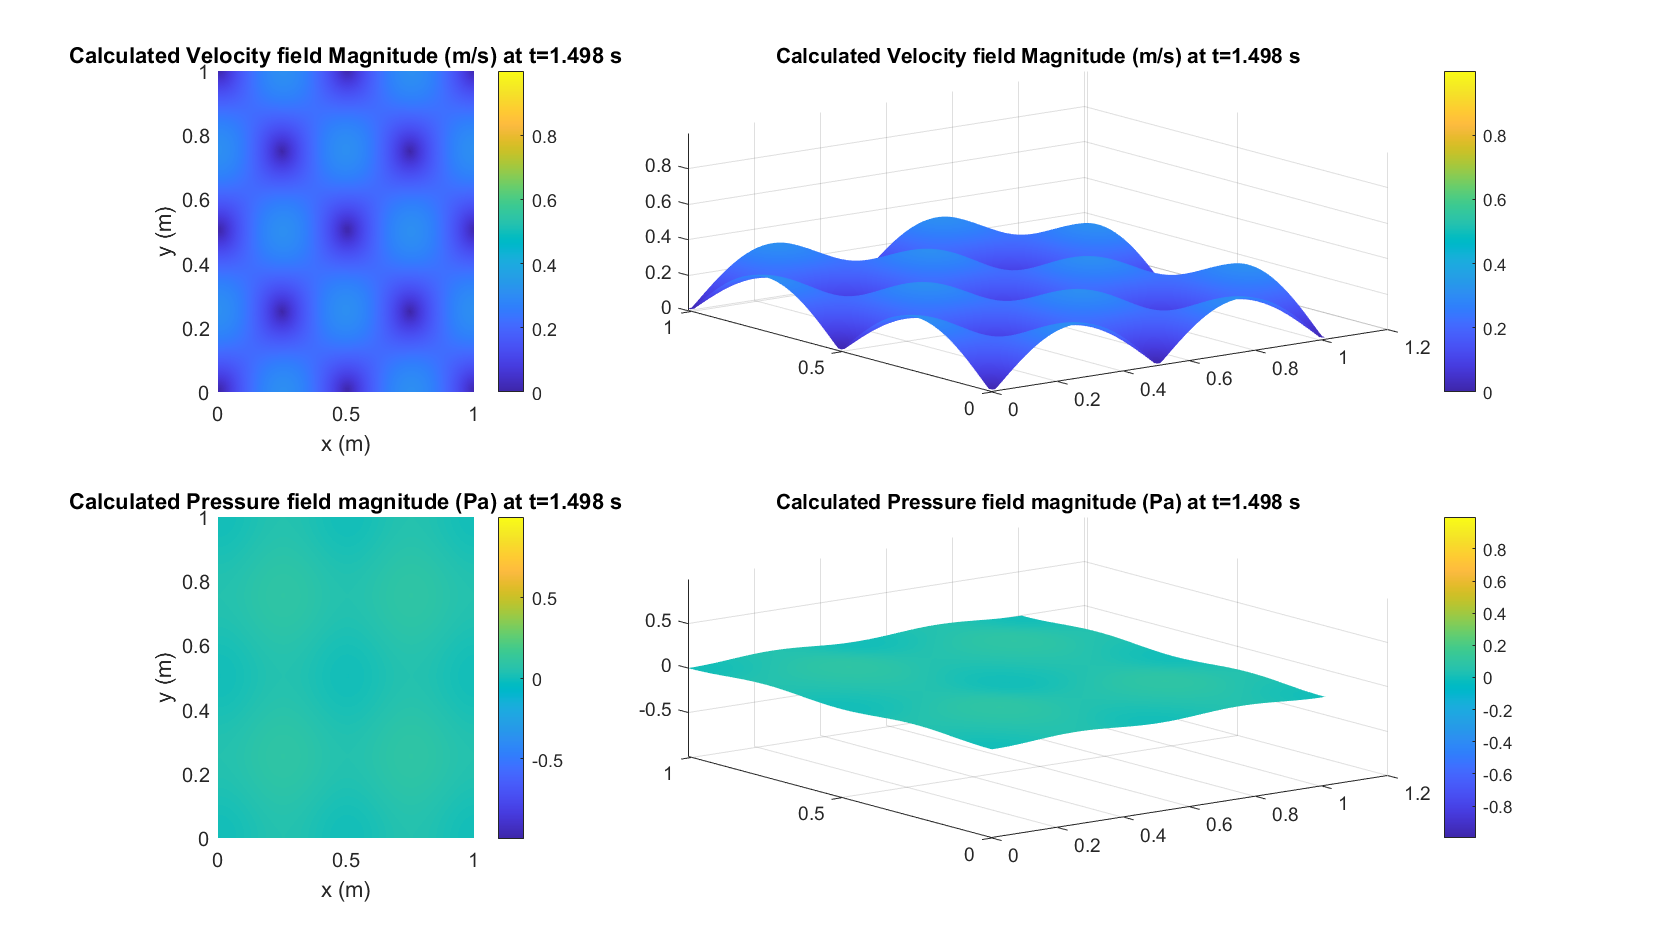
\includegraphics[width=0.6\linewidth]{imatges/calculatedfields.png}
    \caption{Calculated velocity and pressure fields at a point in time.}
    \label{fig:calculatedfields}
\end{figure}

Shows a symmetric, periodic variation in the x-component of velocity across the domain, in line with the initial conditions.

\begin{figure}[H]
    \centering
    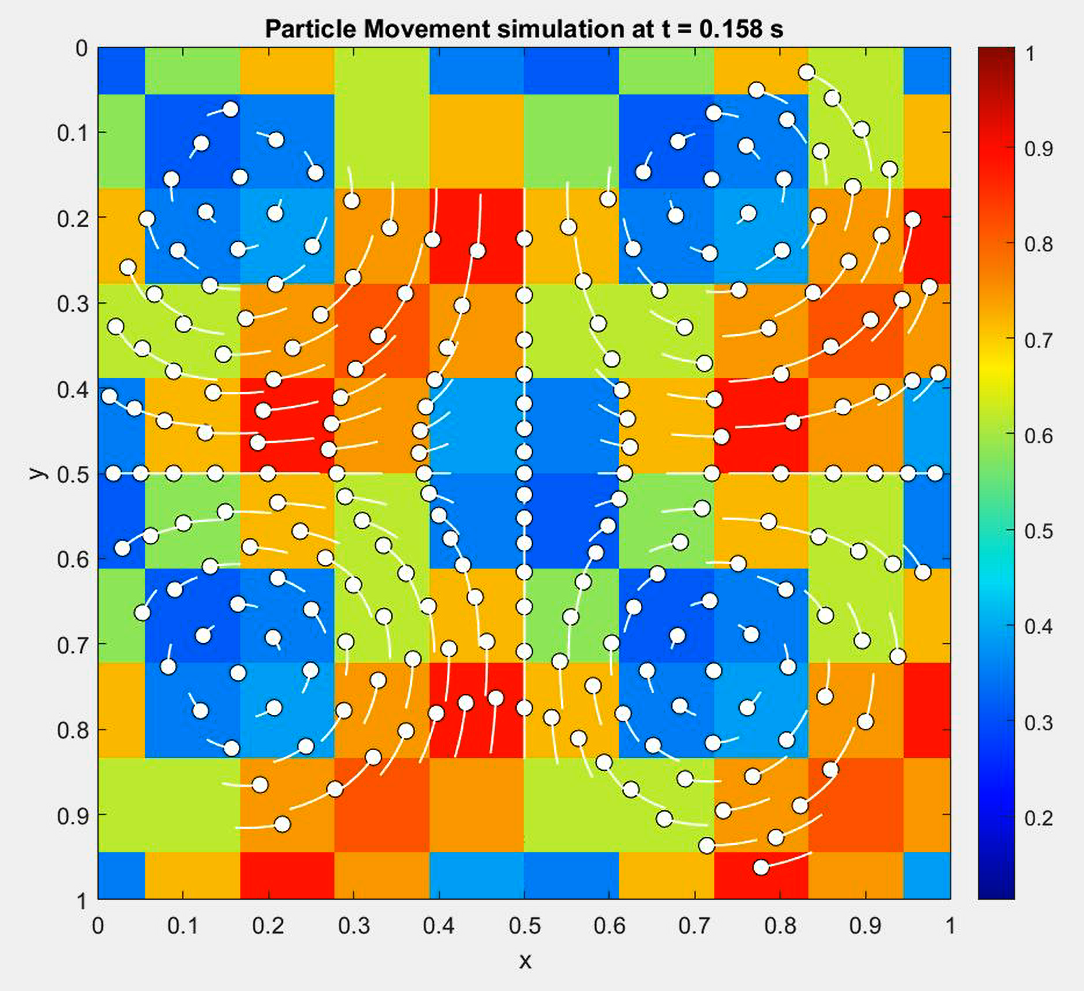
\includegraphics[width=0.6\linewidth]{imatges/particlemovement.png}
    \caption{Screenshot of the particle movement simulation.}
    \label{fig:particlemovement}
\end{figure}
Depicts particle trajectories overlaid on a colored velocity grid, confirming coherent particle motion along the established vector field with evident symmetry and smooth flow paths.